\documentclass[a4paper]{report}
\usepackage{mathtools}
\usepackage{graphicx}

\scrollmode
%
\usepackage{amsmath}
\usepackage{amsfonts}
\usepackage{amssymb}
\usepackage{latexsym}
\usepackage{stmaryrd}
\usepackage{array}
\usepackage{exscale}

\usepackage[driverfallback=hypertex]{hyperref}

%\graphicspath{ {"C:/Users/l_joh/Desktop/tree.jpg"} }

\setcounter{secnumdepth}{2}
\setcounter{tocdepth}{1}

\begin{document}

\title{Reductions for NP-complete problems}

\author{Luke Bevan John\\
  Computer Science Department\\
  Swansea University\\
  Swansea, SA1 8EN, UK
}
\date{}

\maketitle

\begin{abstract}
  Investigation into reductions from SAT to $N$-Queens completion.
\end{abstract}

\tableofcontents


\setcounter{chapter}{-1}

\chapter{TODOS etc.}
\label{cha:todos}

\section{On Latex}
\label{sec:todoslatex}

\cite{lamport94}


\section{Todos}
\label{sec:todostodos}

\begin{enumerate}
\item Consolidate Git-repositories.
\item Next meeting: looking at the C++ code.
  \begin{enumerate}
  \item Testing.
  \item Documentation.
  \item Possibly a Solver
  \end{enumerate}
\item Research: improving the reduction SAT to 3SAT:
  \begin{enumerate}
  \item Examples (complete) and Written out.
  \item Initial concepts.
  \item Literature overview.
  \end{enumerate}
\item Oliver Email\\
 just to summarise the discussion we had:
  \begin{enumerate}
     \item We will focus on the reductions, their implementations and experimental evaluation.
    \item With the implementations, C++ will be learned.
    \item The experimental evaluation can be extended to include the use the machine-learning tools for automatic configuration of the reductions.\\ \\ Oliver
  \end{enumerate}
\end{enumerate}




\chapter {Introduction}
\label{cha:Introduction}

\section{Background}
\label{sec:Background}



\chapter{SAT to 3SAT}
\label{cha:sat13}

\begin{enumerate}
\item \cite{Cook1971NP}
  \begin{enumerate}
  \item Theorem proves that every language in co-NP can be reduced to TAUT.
  \item The proof of Theorem 1 actually shows that SAT (for CNF) is NP-complete.
  \item Theorem 2 shows that 3-CNF (every clause has length at most 3) is NP-complete. This happens by splitting up a clause $x_1 \vee \dots \vee x_s$ into
    \begin{displaymath}
      v \vee x_1 \vee x_2, \quad \neg v \vee x_3 \vee \dots \vee x_s.
    \end{displaymath}
XXX proof of correctness YOURSELF

a couple of sentences WHAT is to be proven

a couple of sentences for the arguments

  \item This all in a different language.
  \end{enumerate}

\end{enumerate}

$\phi$ = $( x_1 \wedge x_2 ) \vee (\neg x_1 \vee x_3) \wedge \neg x_2$ 
\\
\\
\\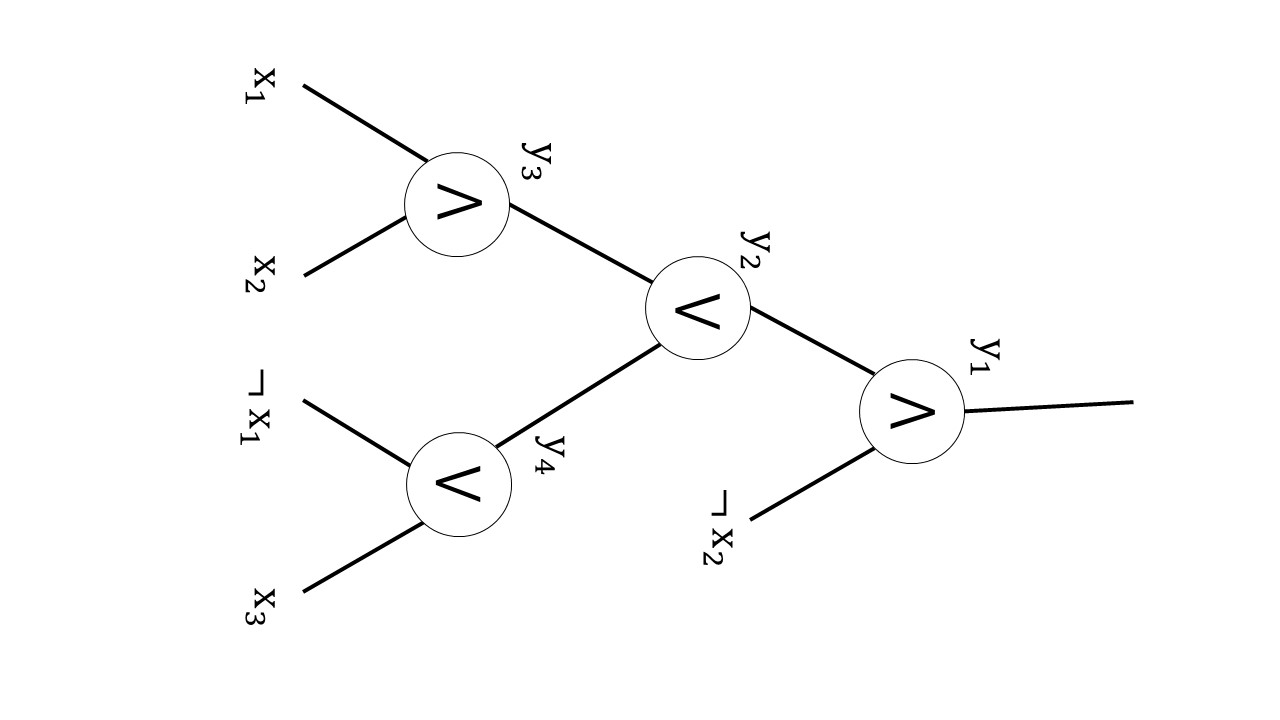
\includegraphics[scale = 0.3 , angle = 90]{tree.jpg}\\
$\phi ' $
\begin{tabular}{|c|}
\hline
$ = y_1 \wedge$ $(y_1$  $\iff$ $( y_2 \wedge \neg x_2))$   \\
$(y_2$  $\iff$ $( y_3 \vee  y_4))$   \\
$(y_3$  $\iff$ $( x_1 \wedge  x_2))$   \\
$(y_4$  $\iff$ $( \neg x_1 \vee  x_3))$   \\
\hline
\end{tabular}\\
\\
\\%$p \iff q \equiv (p \wedge q) \vee ( \neg p \wedge \neg q)$
\\ 

truth table for biconditional statment\quad$ p \iff q $\\

\begin{tabular}{|c|c|c|}
\hline
p & q&  \\
\hline
T & T & T \\
T&F&F\\
F&T&F\\
F&F&T\\
\hline
\end{tabular}\\
\\
\\

\begin{tabular}{ |c|c|c|c|c| }
\hline
p&
\multicolumn{2}{|c|} {q}\\
\hline
$y_1$&$y_2$&$\neg y_2$&Clause 1\\
\hline		
1&1&0&	FALSE*\\
1&1&1&	TRUE\\
1&0&0& 	FALSE*\\
1&0&1&	FALSE*\\
0&1&0&	TRUE\\
0&1&1&        FALSE*\\
0&0&0&	TRUE\\
0&0&1&	TRUE\\
\hline
\end{tabular}\\

$\neg C_1 = (y_1 \wedge y_2 \wedge x_2) \vee (y_1 \wedge \neg y_2 \wedge x_2) \vee (y_1 \wedge \neg y_2 \wedge \neg x_2) \vee (\neg y_1 \wedge y_2 \wedge \neg x_2)$\\
\\
\begin{tabular}{|c|}
\hline
Demorgans Law\\
$\neg( p \wedge q ) = \neg p \vee \neg q$\\
$\neg( p \vee q ) = \neg p \wedge \neg q$\\
\hline
\end{tabular}\\
\\
$CNF\quad C_1 = (\neg y_1 \vee \neg y_2 \vee \neg x_2) \wedge ( \neg y_1 \vee y_2 \vee \neg x_2) \wedge (\neg y_1 \vee y_2 \vee x_2) \wedge ( y_1 \vee \neg y_2 \vee x_2) $\\
\\
\\
\begin{tabular}{ |c|c|c|c|c| }
\hline
	
$y_2$&$y_3$&$y_4$&Clause 2\\
\hline		
1&1&0&	TRUE\\
1&1&1&	TRUE\\
1&0&0&	FALSE*\\
1&0&1&	TRUE\\
0&1&0&	FALSE*\\
0&1&1&	FALSE*\\
0&0&0&	TRUE\\
0&0&1&	FALSE*\\
\hline
\end{tabular}\\



\section{3SAT to 1-in-3-SAT}
\label{sec:3satto13}



\bibliographystyle{plainurl}
\bibliography{Bibliography}

\end{document}